\documentclass[12pt,twoside]{article}
\usepackage{light}
\usepackage{subfigure}
\usepackage{graphicx}
\hidesolutions
%\showsolutions

%Solutions are currently incorrect
\begin{document}
\begin{problem}{15} 
Use the web graph below to answer parts (a), (b), and (c) of this question. The pagerank of vertex $i$ can be written as $p_i$. Assume each webpage starts out with a million dollars.
\begin{figure}[h]
\begin{center}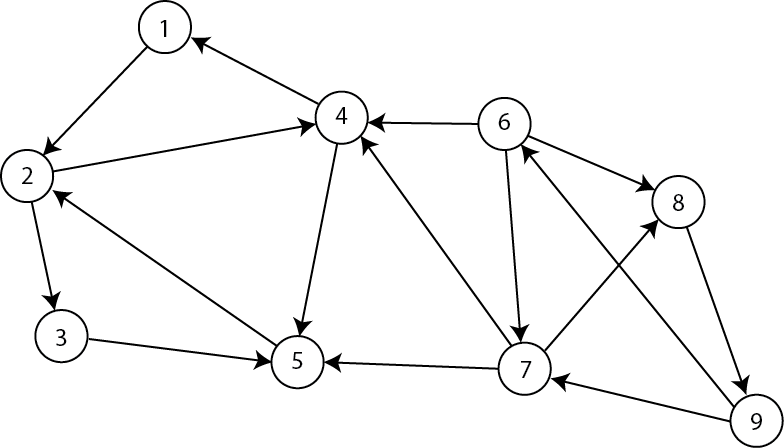
\includegraphics[width=12cm]{pagerank.png}\end{center}
\caption{Web Graph}
\end{figure}

\bparts

\ppart{6} Compute the first two iterations of PageRank, starting
from uniform PageRank values of a million across all vertices.
\solution{
}

\ppart{5} For $\vec{p}'$ in terms of $\vec{p}$ can be written as a matrix product: $\vec{p}' = W\vec{p}$, for some matrix $W$, which is the \emph{update matrix}. Find the update matrix.
\solution{
}

\ppart{5} Calculate the stationary values for the web graph.
\solution{
 }

\eparts
\end{problem}
\end{document}
